\chapter{Prototype tests at IPHI}
\chaptermark{Prototype tests at IPHI}
\cleardoublepage

\minitoc

\section{Introduction}
\begin{refsection}
  \label{ch4:Introduction [C]}
  The simulations presented in the previous chapter show that the profile measurement with IPM may matches the ESS requirement. However, some critical points, mainly about the choice of the readout, are not fully clarified, so the feasibility must be proven experimentally. From the results of the simulation, we converge to a first prototype design. Designing and testing prototypes is also a great opportunity to validate the simulations and earn feedbacks before the production phase. The following chapter presents the different prototypes that has been developed and tested as well as the results obtained. In fact, the chapter follows closely the real chronology of the cNPM project.

  The feasibility of silicon detection has been checked. A small test bench has been developed and installed in a ion implanter facility. The test has been done with a tailored silicon detector kindly provided by the CERN-BI team. The result and it consequence on the project will be discussed briefly.

  Then, a full test bench has been designed including several IPM and reference measurement. The different levels of integration for each component of the test bench will be described in order to give a global overview.

  Finally, the test bench has been installed on a 3 MeV accelerator. Two test campaign has been done and the different IPMs have been tested and characterized. The setups and most of the results will be presented in this chapter.

  \section{Preliminary tests of silicon detector [C]}
  The readout using silicon detector seems very promising but detection is not assured for ions at low energies. It requires significant development in terms of electronics: complex PCB design, placement and alignment of the chips, wire bonding, development of a backend electronic. Therefore, we decided to test a proof of concept before directly developing a complete IPM with silicon detector. If the test shows that detection with ions is possible then this solution can be considered at ESS, otherwise it will be discarded. Therefore, a low energetic ion source is necessary for testing the silicon method.

  \subsection{IRMA [C]}
  An implanter is a small ion accelerator used to implant various elements into a target substrate. The depth of the implementation is proportional to the ion acceleration \footnote{See section \ref{chap3:sec_particle_in_matter} and \ref{chap3:low_energy} in the previous chapter}. This kind of sources is particularly useful for material and irradiation sciences, and it may be the most efficient way to test the silicon detectors for us.

  The IRMA implanter \cite{Chaumont1981} relies on a Bernas-Nier source \cite{Paris1981} for creating a plasma from injected gas. The plasma is then extracted and charge filtered by the means of a magnet. The post acceleration is performed by an electrostatic tube. Finally, a set of steerers allows a fine beam scanning on the target. The IRMA implanter can accelerate a large number of elements between 5 to 190 keV with currents about uA scale. Fig. \ref{chap4:IRMA_facility} presents a schematic representation of IRMA and a picture of the facility.
  \begin{figure}[!ht]
	\begin{subfigure}{0.5\textwidth}
		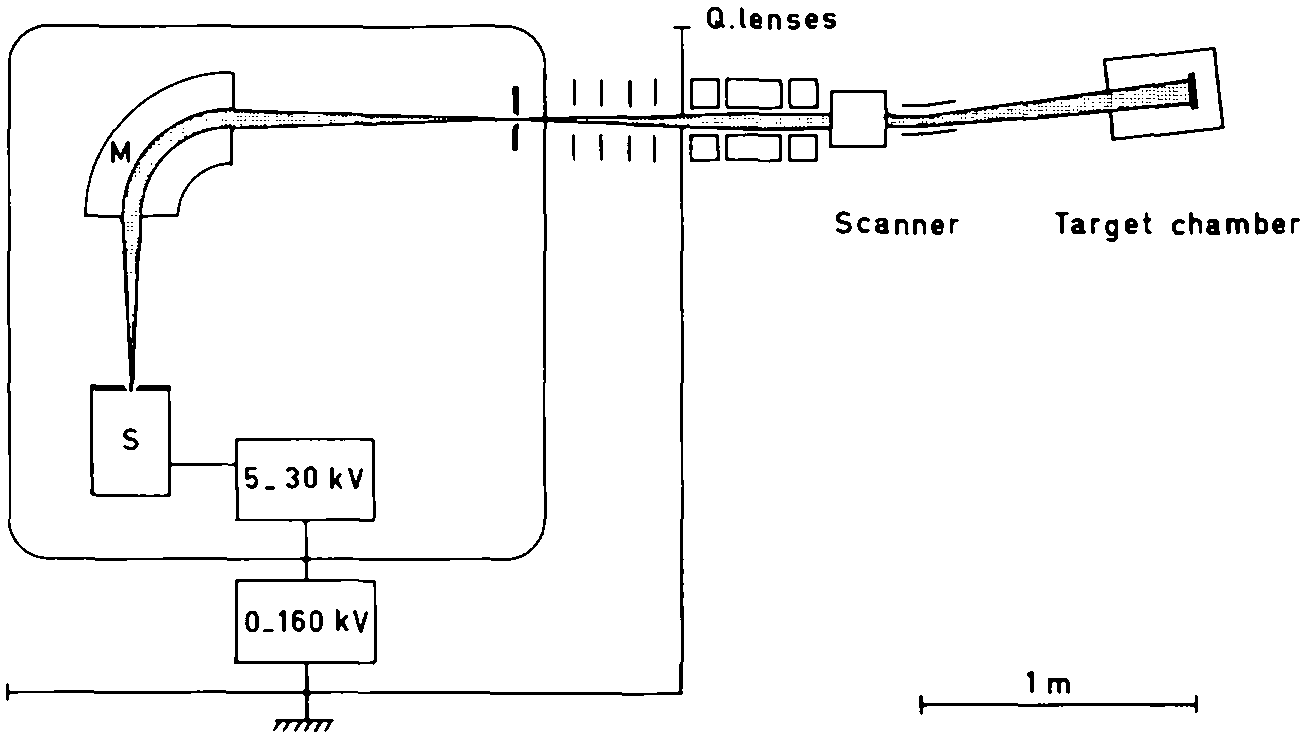
\includegraphics[width=\textwidth]{04_IPHI_Test/figures/fig000_IRMA01.png}
		\caption{}
		\label{}
	\end{subfigure}
	~
	\begin{subfigure}{0.5\textwidth}
		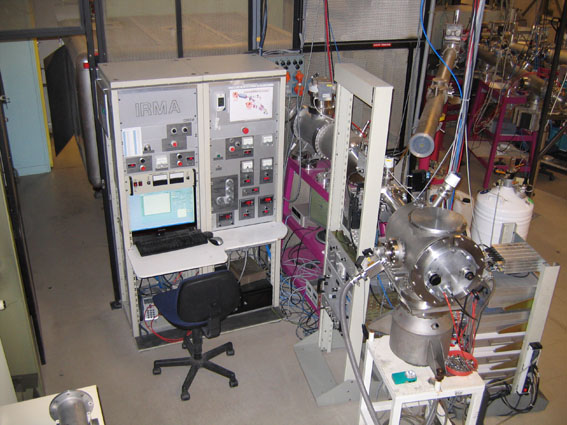
\includegraphics[width=\textwidth]{04_IPHI_Test/figures/fig000_IRMA02.jpg}
		\caption{}
		\label{}
	\end{subfigure}
	\caption[IRMA installation]{IRMA installation}
	\label{chap4:IRMA_facility}
\end{figure}

  
  \subsection{Test setup [En cours de rédaction]}
  \cite{advacam2019}
  \cite{Kraus2011}

  \begin{figure}[!ht]
	\begin{subfigure}[t]{0.5\textwidth}
		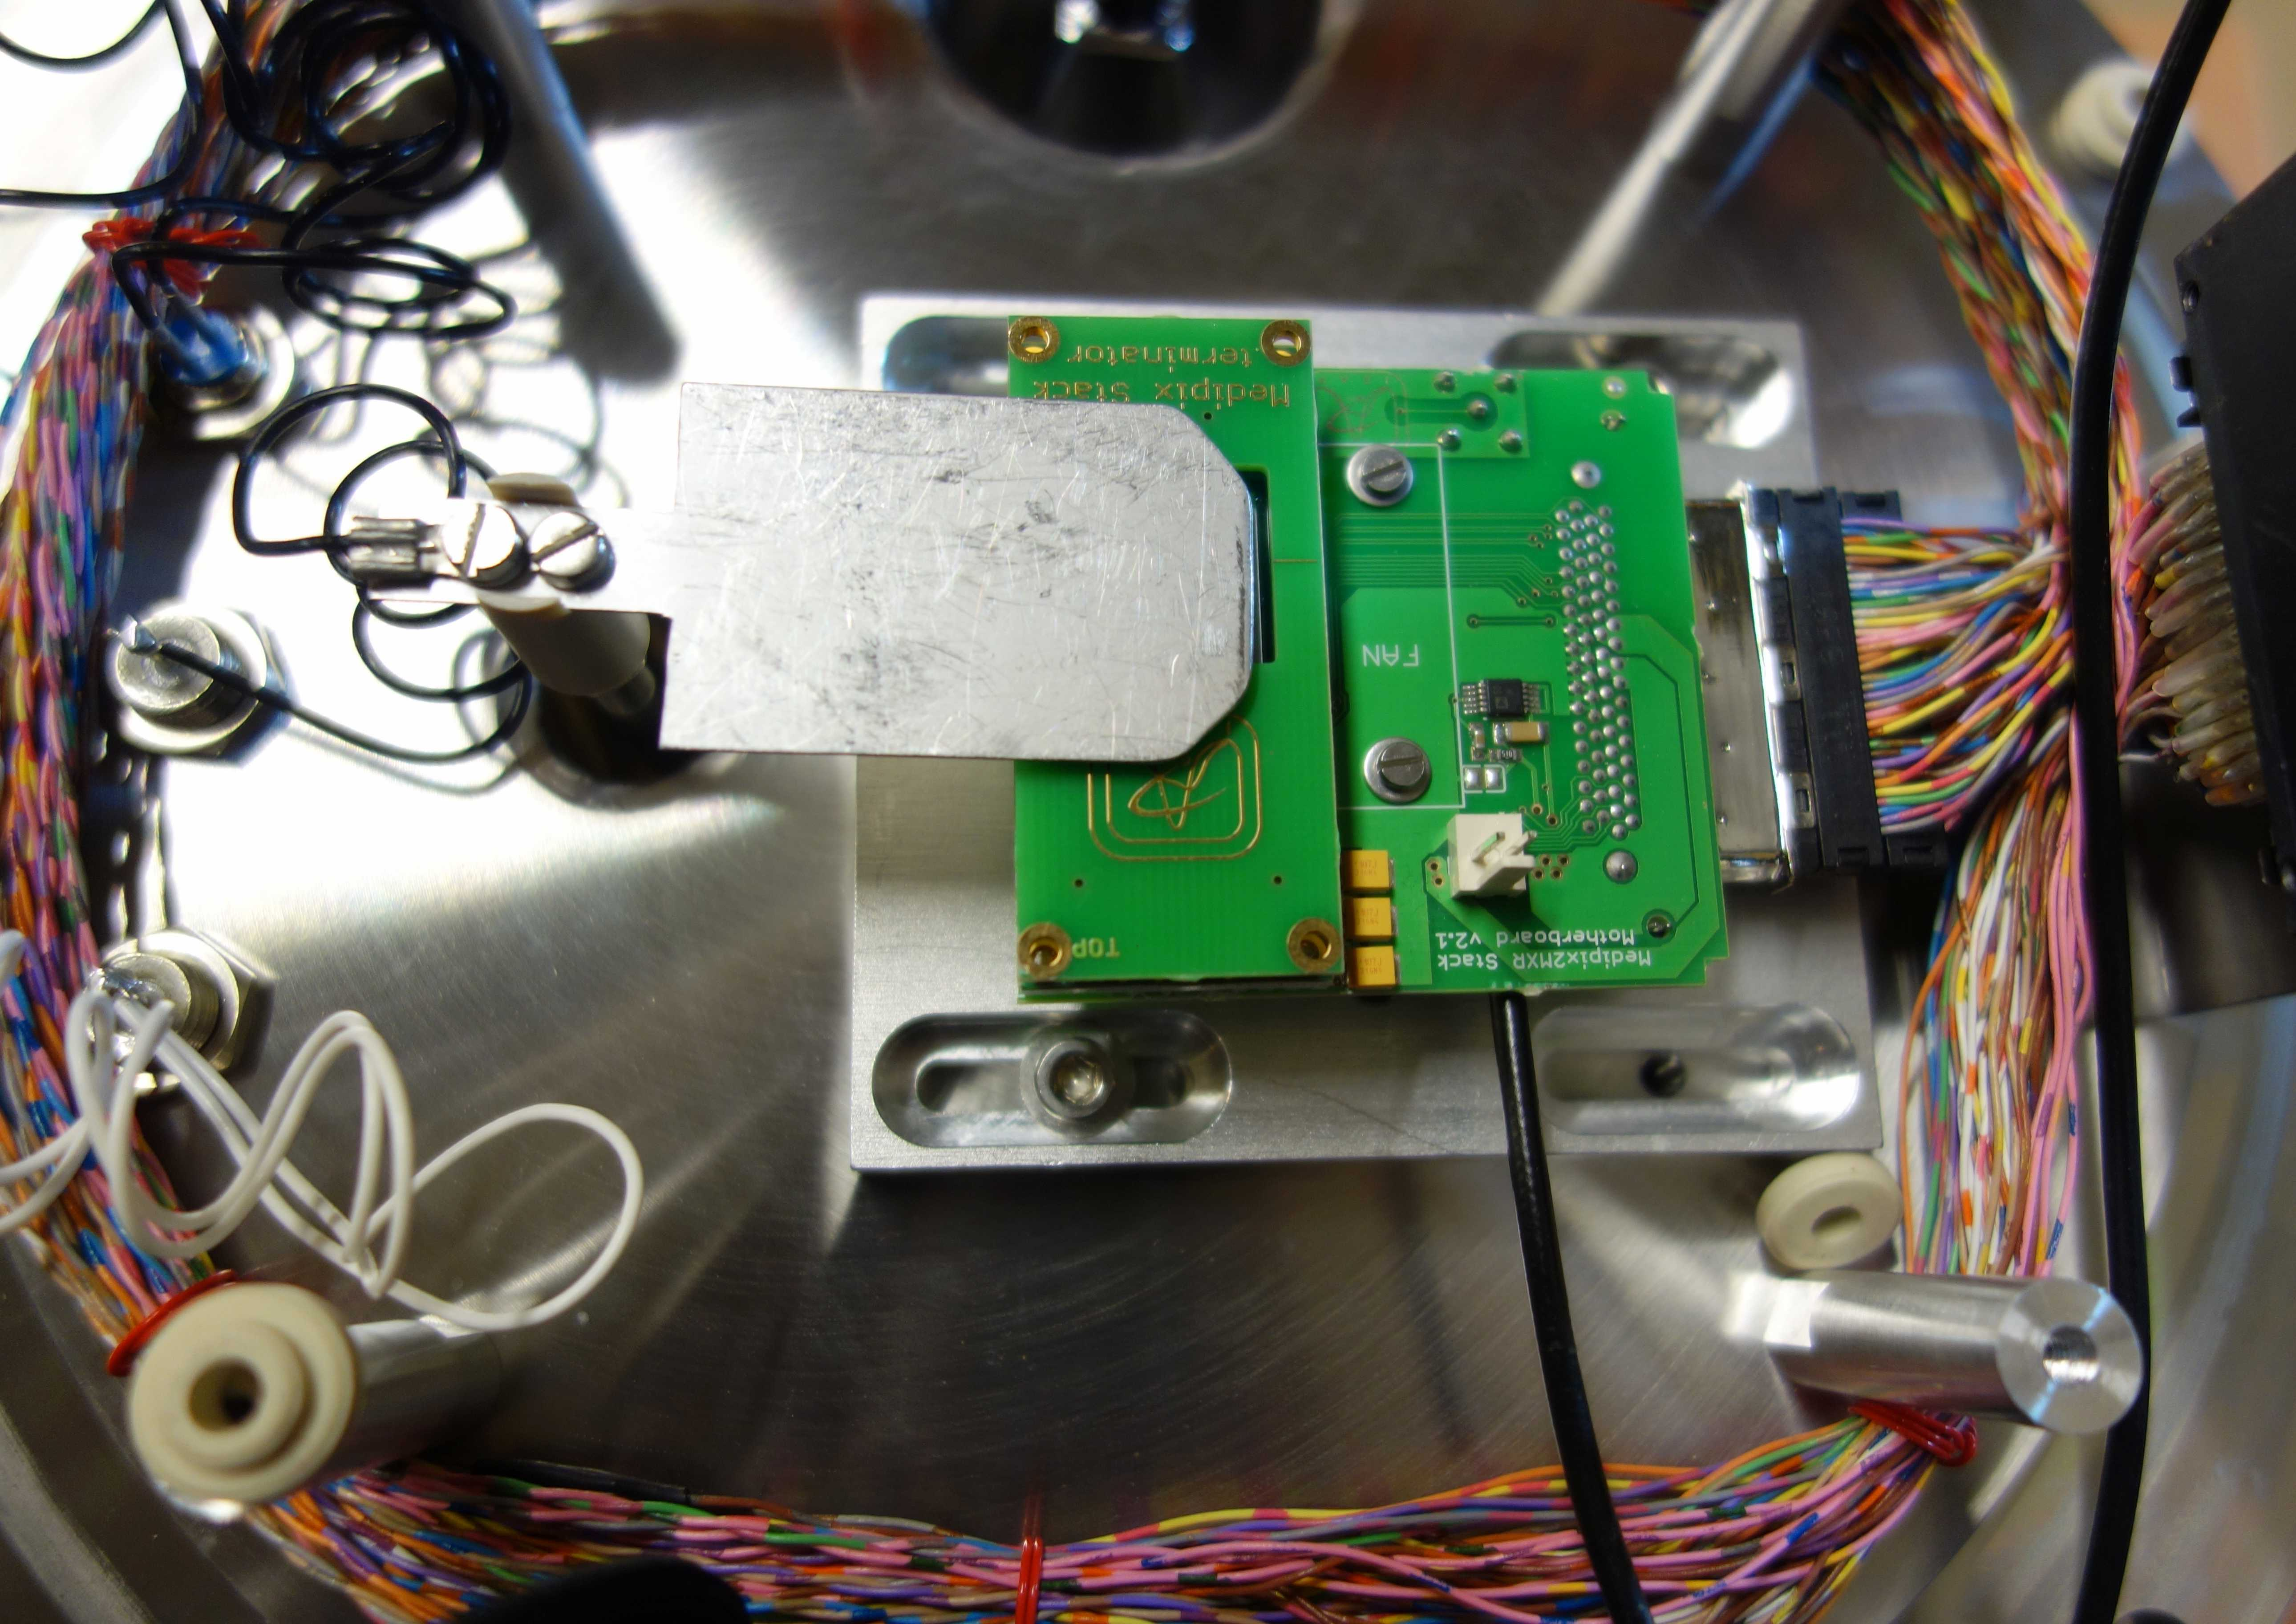
\includegraphics[width=\textwidth]{04_IPHI_Test/figures/fig000_IRMA_setup01}
		\caption{The TimePix chip is just behind the Faraday cup.}
		\label{}
	\end{subfigure}
	~
	\begin{subfigure}[t]{0.5\textwidth}
		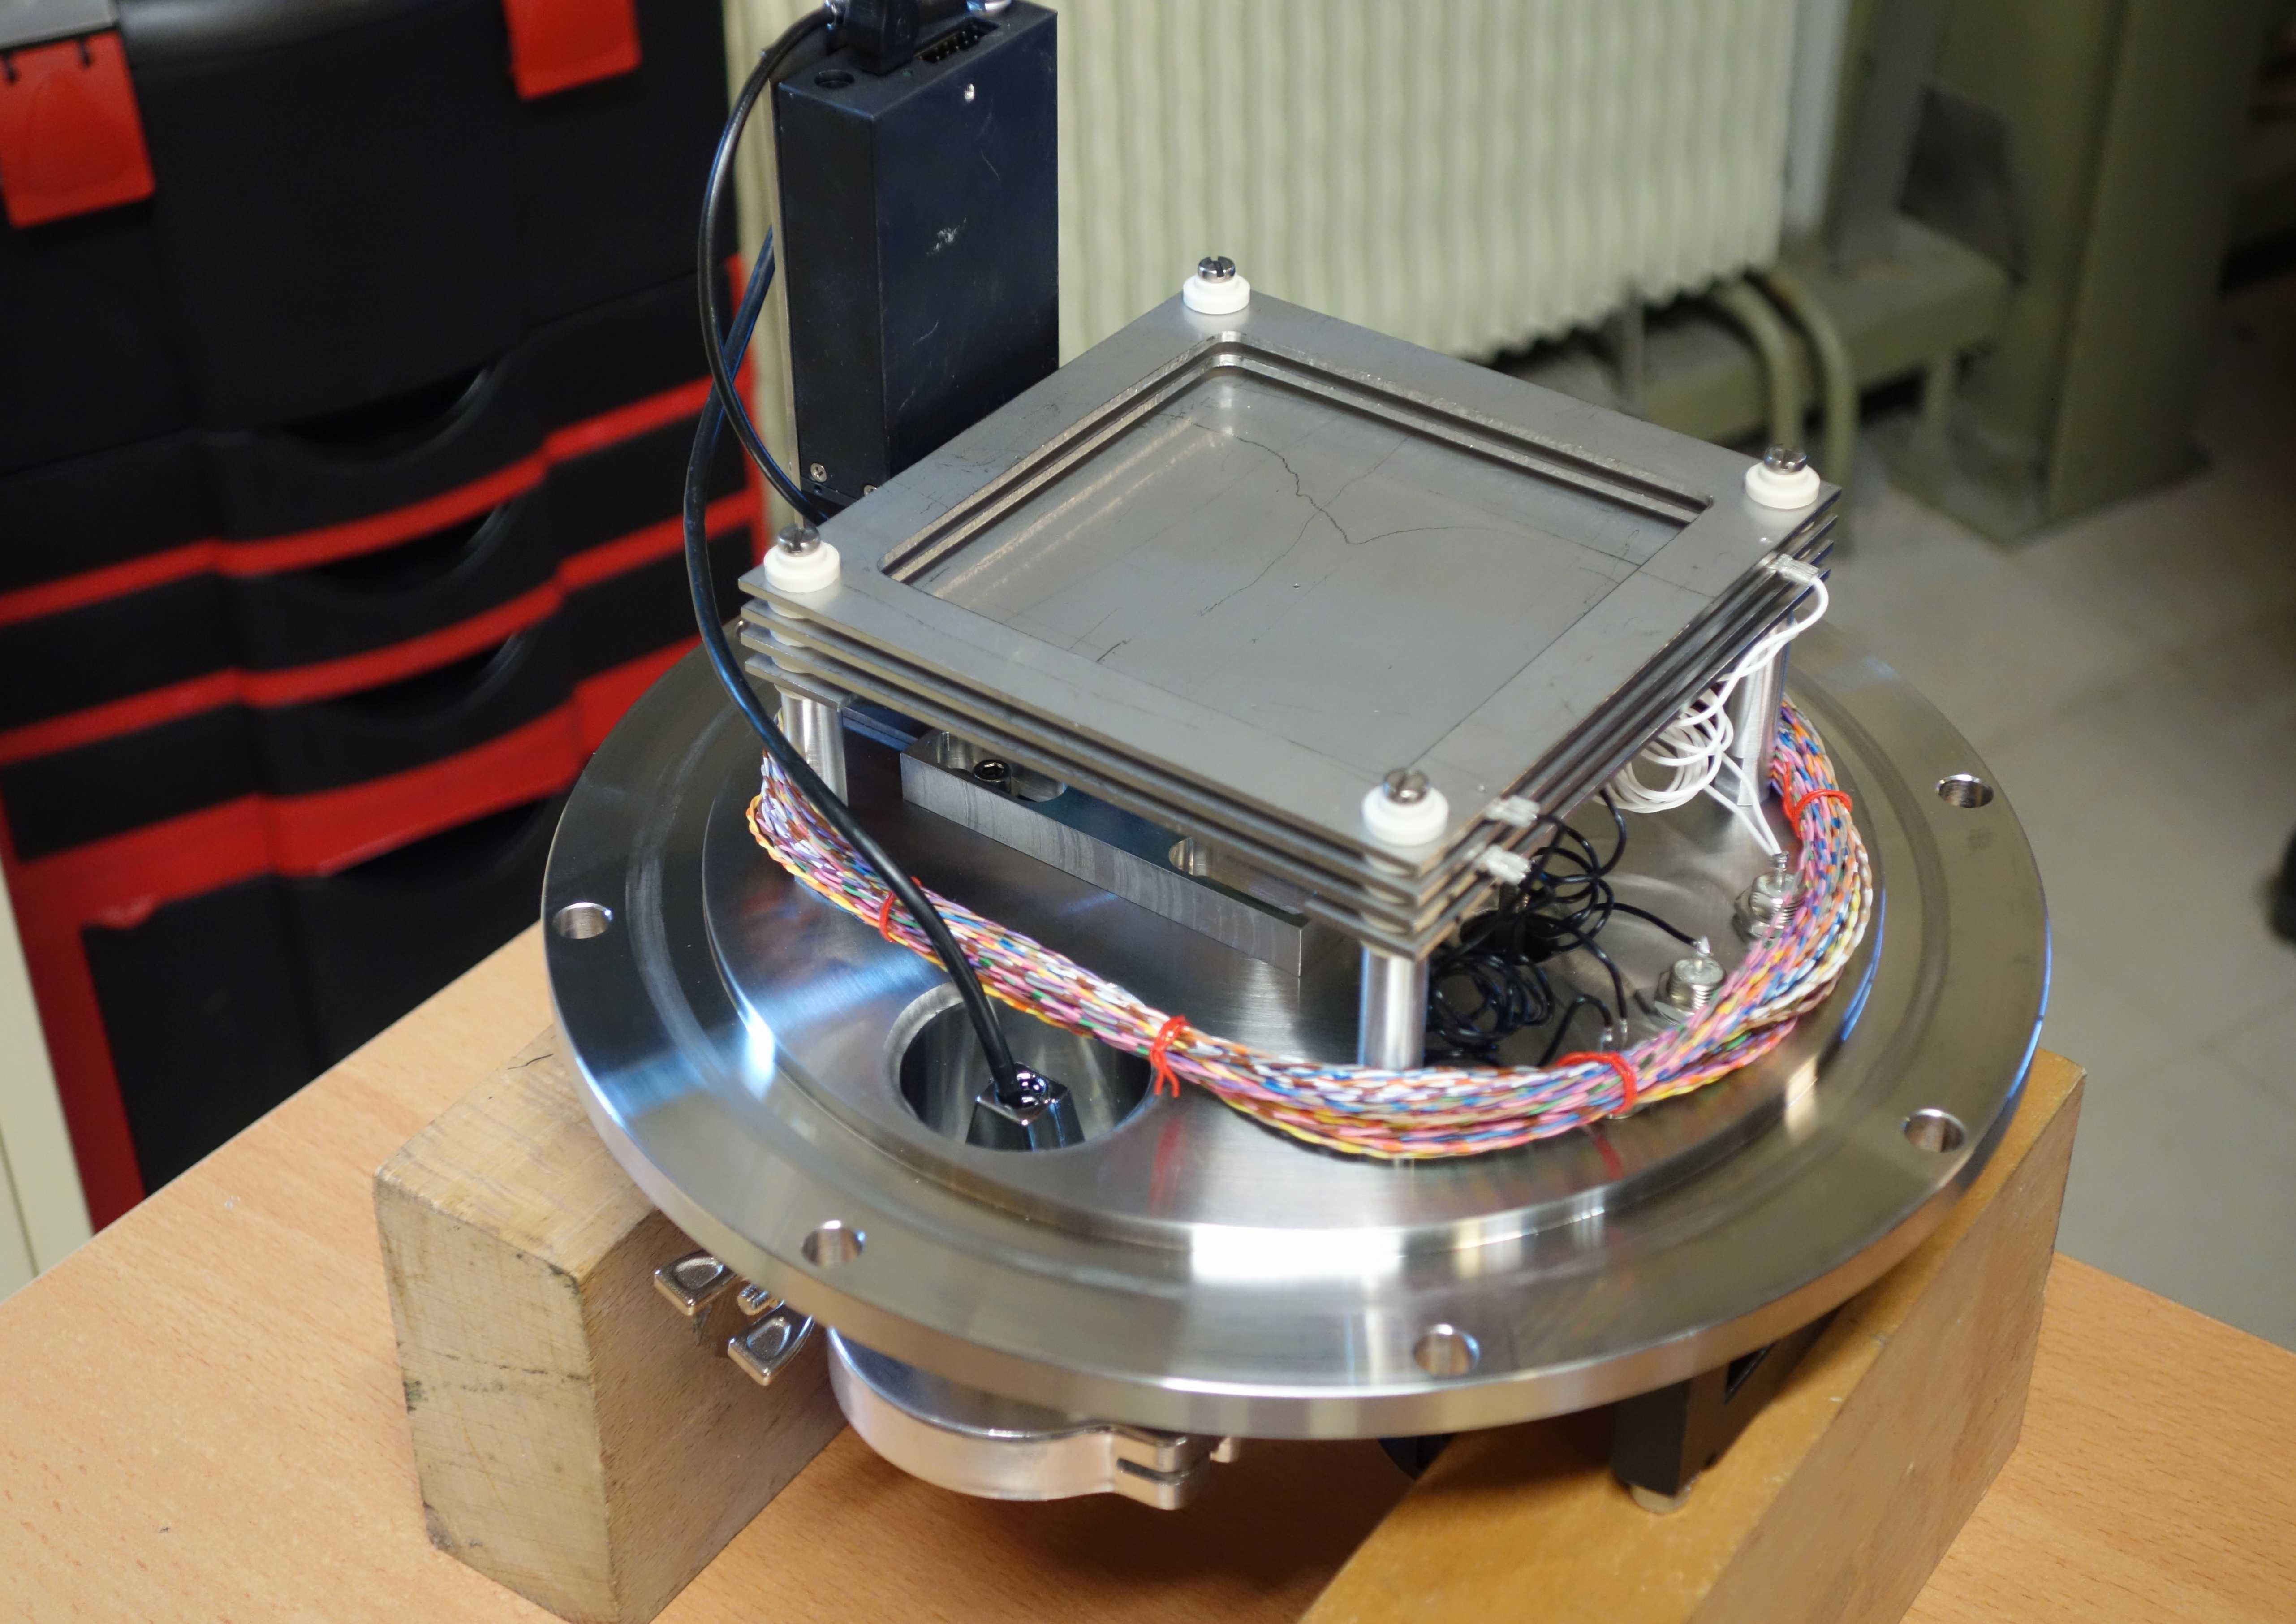
\includegraphics[width=\textwidth]{04_IPHI_Test/figures/fig000_IRMA_setup02}
		\caption{A plate with a drilled hole reduced the incoming current. The beam is scanned on the plate.}
		\label{}
	\end{subfigure}
	\caption[IRMA setup]{IRMA setup. A dedicated test bench has been developed for testing the TimePix chips.}
	\label{chap4:IRMA_setup}
\end{figure}

  \subsection{Results and limitations [En cours de rédaction]}
  
  \begin{figure}[!ht]
	\begin{subfigure}{0.25\textwidth}
		\includesvg[width=\textwidth]{04_IPHI_Test/figures/fig000_IRMA_15keV}
		\caption{ToT image at $15\,\mathrm{keV}$}
		\label{}
	\end{subfigure}
	~
	\begin{subfigure}{0.25\textwidth}
		\includesvg[width=\textwidth]{04_IPHI_Test/figures/fig000_IRMA_12keV}
		\caption{ToT image at $12\,\mathrm{keV}$}
		\label{}
  \end{subfigure}
  ~
  \begin{subfigure}{0.5\textwidth}
		\includesvg[width=\textwidth]{04_IPHI_Test/figures/fig000_IRMA_sweep}
		\caption{Total signal on the sensor with respect to the ion energies.}
		\label{}
  \end{subfigure}
	\caption[Main results from IRMA tests with $H_{2}^{+}$ ions]{Main results from IRMA tests with $H_{2}^{+}$ ions.}
	\label{chap4:IRMA_Si}
\end{figure}

  Few days after the test, the integrity of the sensor has been test by illuminating it with an UV-VIS LED (peak emission at 365nm). A zone in the matrix and it is visible in Fig. \ref{}. 
  This zone is exactly in the same place as the one bombarded by the ions. The sensor has been probably deteriorated by the high current of IRMA. Unfortunately it is not possible to accurately estimate the number of ions that have been sent to the sensor and the nature of the damage is unknown. Note that the gain has increased in the irradiated region.

  We decided to not go further with silicon detectors for all the previous reasons. The cost of development of a silicon solution is not worth considering the possible risks of non detection. We would like to remain that the experiment has been done to quickly check the feasibility and it suffers from several limitations. Firstly the detector was not triggered, during short acquisitions pulse only very few data were taken in coincidence with the beam, therefore long acquisitions have been favored reducing the uncertainty only on the first and last pulse. The second uncertainty comes from the beam scanning. We noticed that, sometimes, the beam could pass through the hole more than once for a same scanning cycle. This means that the number of charge is collected by the TimePix is more than expected for an acquisition.

  We hope that further testing will be done to fully determine the detection limit of this method with ions and investigate more on the ion damaging. Since our tests TimePix 3 has completely replaced its ancestor. This version provides the ability to measure at same time the ToT and ToA, higher timing resolution and efficient data protocol. As well, the reading electronics has been improved allowing advanced triggering option of the chip.
  
  \section{IPM design overview[En cours de rédaction]}
  \subsection{IPM [En cours de rédaction]}
  \subsection{MCP [En cours de rédaction]}
  %\begin{table}[ht]
  \centering
  \caption[The main characteristics of MCPs used during the beam tests]{The main characteristics of MCPs used during the beam tests. MCPs from Hamamatsu has the same characteristics except that one has a phosphorus screen as readout.}
  \label{chap4:MCP_Phosphor}
  \begin{tabular}{llll}
    \toprule
                     & Hamamatsu         & Photonis 1                  & Photonis 2                  \\
    \midrule
    Active radius    & $40\,\mathrm{mm}$           & $40\,\mathrm{mm}$           & $40\,\mathrm{mm}$           \\
    Channel diameter & $12\,\mathrm{\mu m}$        & $10\,\mathrm{\mu m}$        & $25\,\mathrm{\mu m}$        \\
    Channel pitch    & $15\,\mathrm{\mu m}$        & $12\,\mathrm{\mu m}$        & $32\,\mathrm{\mu m}$        \\
    OAR              & $60\,\mathrm{\%}$           & $55\,\mathrm{\%}$           & $45\,\mathrm{\%}$           \\
    Bias angles      & $8\,\mathrm{\textdegree{}}$ & $8\,\mathrm{\textdegree{}}$ & $8\,\mathrm{\textdegree{}}$ \\
    \midrule
    Screen type      & $P43$                  & $P46$                       & -                           \\
                     & $Gd_{2}O_{2}S:Tb$           & $Y_{3}Al_{5}O_{12}:Ce$      &                             \\
    Gain relative    & $1$                      & $0.3$                       & -                           \\
    Wavelength       & $545\,\mathrm{nm}$      & $530\,\mathrm{nm}$          & -                           \\
    Decay time range & $\mathrm{ms}$           & $\mathrm{\mu s}$            & -                           \\
    \bottomrule
  \end{tabular}
\end{table}
  \subsection{Camera [C]}
  A vision system is necessary to record light from the phosphorus screen.
  A camera with a lens should be sufficient in our case.

  % Sensor
  Sensor is the core component of a camera so it's better to choose the sensor first with respect to the requirements.
  For our application high resolution is not mandatory, so pixels could be relatively big in order to increase light collection and dynamic range.
  Sony IMX249 fits well with these prerequisites. It's a consumer CMOS sensor with relatively big pixels and low noise.
  Its EMVA characteristics are summarized in the Table \ref{tab:IMX249} \cite{emva2010}.
  \begin{table}[!h]
  \centering
  \caption{Main features of the Sony IMX249 sensor}
  \label{tab:IMX249}
  \begin{tabular}{ll}
    \toprule
    Resolution           & 1936 (H) * 1216 (V)  \\
    Pixel size           & 5.86 $\mu m$         \\
    Sensor diagonal size & 13.4 mm (Type 1/1.2) \\
    Well capacity        & 32000 e-             \\
    Dynamic Range        & 70 dB                \\
    QE at 525 nm         & 70 \%                \\
    Electrons noise      & 6.8 $e^{-}$          \\
    ADC                  & 8, 10 or 12 bits     \\
    Max framerate        & 30 fps               \\
    \bottomrule
  \end{tabular}
\end{table}

  % Camera
  AlliedVision, Basler and FLIR propose several cameras based on the IMX249 sensor with different interfaces, features, form factors, prices and availability.
  We restricted our choice to GigE cameras since they allow long cable length and Power over Ethernet (PoE) which are quite useful features for an accelerator experiment.
  At the end we choose the FLIR Blackfly-PGE-23S6M-C \cite{blackfly2019}.

  % Lens
  The last step is the choice of a correct lens for the camera.
  Unfortunately lens suppliers doesn't provide full characteristics of their lenses, hence only the thin lens approximation has been considered.
  Distance from back of phosphorus screen to external air-side of viewport is 247mm. Active area radius of our MCPs is around 25mm thus magnification, with respect to a sensor size of 11.34 mm, should be at least 0.2268.
  Table \ref{tab:lens_magnification} shows magnification for several focal length. A focal length of 50 mm fits very well with our configuration.
  \begin{table}[!h]
  \centering
  \caption[Magnification for several common focal lengths]{Magnification for several common focal lengths, at a working distance of $247\,\mathrm{mm}$.}
  \label{tab:lens_magnification}
  \begin{tabularx}{1\textwidth}{lllllllll}
    \toprule
    Focal length ($\mathrm{mm}$) & $5$    & $15$    & $28$    & $35$    & $50$    & $75$    & $100$  & $150$   \\
    Magnification     & $0.02$ & $0.069$ & $0.127$ & $0.165$ & $0.255$ & $0.436$ & $0.68$ & $1.546$ \\
    \bottomrule
  \end{tabularx}
\end{table}

  Lenses with 50mm focal length are rather standard and commercially available at moderate cost. In addition these lenses have a large numerical aperture (or small F-number) so they provide a large photon capture efficiency.

  \subsection{Strips [En cours de rédaction]}
  \subsection{CARAMEL board and FASTER system [En cours de rédaction]}
  \cite{ddc316}\cite{caramel2013}\cite{faster2013}\cite{rhb2012}
  \subsection{Control System [C]}
  The whole ESS Control System (CS) will rely on the EPICS (Experimental Physics and Industrial Control System) toolkit. The ESS CS team has specified its own EPICS standards to ensure the sustainability of the control system over the years. We will also test our IPMs in an accelerator that is EPICS compatible. Therefore, EPICS has some importance to our project and we tried to use it as much as possible for our prototypes. In this section we will briefly describe EPICS and how we have integrated our test bench.

  EPICS provides a set of tools and protocols to facilitate the integration of control system \cite{epics2019}. Originally developed for real-time systems, EPICS now supports many platforms. EPICS has become an open source project in 2004, since many laboratories and collaborations have contributed to EPICS.
  One of most important component of EPICS is the Channel Access (CA). In few words, it is a protocol that defines how the data are exchanged between clients and servers on a network. A server provides Processes Variables (PV) to clients. A PV is a useful data (for instance a current, a voltage or a temperature) associated with metadata (timestamp, units). A client can access and edit a PV value by knowing its name. In practice a server is often an hardware controlled by software, often called software Input / Output Controller (softIOC). A client is for instance an operator interface (OPI) which allows to view and modify the PV from one or more softIOCs.

  The whole system is almost fully compatible with the version 3.16 of EPICS base. The PointGrey GigE cameras are well supported by the AreaDetector module \cite{ad2019}. A custom plugin, developed by ESS, perform an gaussian fit on the profile every image. Raw images are saved into HDF5 files \cite{hdf5}. It allows to pack  various datasets together, for instance the raw IPM images with some beam information.
  Since all high voltage power supplies have their own SPCI Ethernet interface, thus a simple softIOC with StreamDevice\cite{streamdevice2019} was enough to control and monitor them.
  Three OPIs have been developed in order to control cameras, power supplies and geobrick. They run under BOY module of the ESS Control System Studio version 4.5. An Archiver Appliance records and saves slow process variables from the power supplies, the vacuum systems and the accelerator \cite{archiver2019}.

  \begin{figure}[!ht]
	\begin{center}
		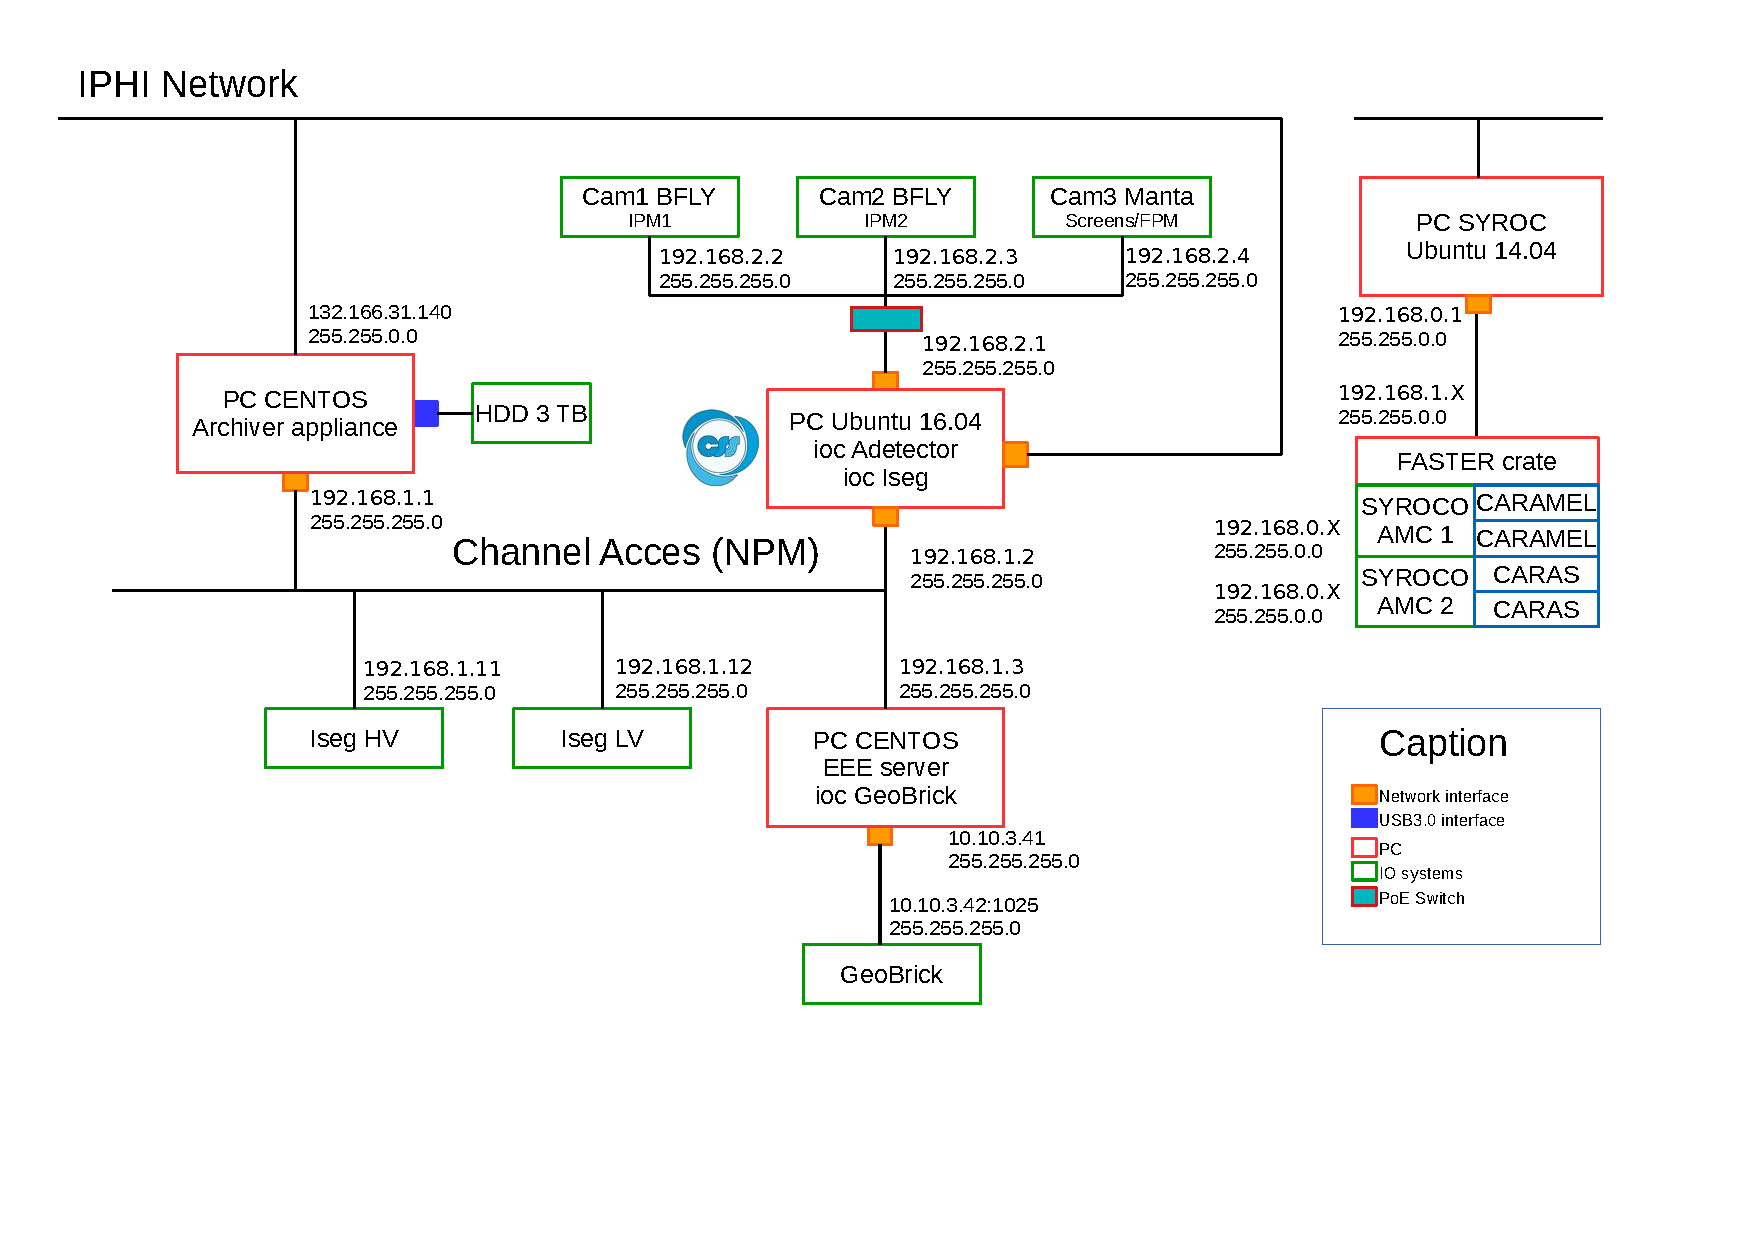
\includegraphics[width=\textwidth]{04_IPHI_Test/figures/fig000_EPICS_IPHI.pdf}
	\end{center}
	\caption[EPICS network setup during beam tests]{EPICS network setup during beam tests.}
	\label{chap4:EPICS_IPHI}
\end{figure}


  \subsection{Test bench [C]}
  A test bench has been also developed in order to test the prototypes. The bench can be split into two different independent parts.

  The first part (upstream) tries to mimic the ESS LWU chamber on which two IPMs can be inserted. The idea is to be close to the ESS conditions in term of high voltages and electrical fields. The second part (downstream) offers one more IPM slot and two viewports for reference measurements in order to compare with the IPMs. Fig. \ref{chap4:Testbench} presents a technical drawing of the test bench. One can see the resemblance of the upstream part with the LWU vessel previously shown in Fig. \ref{chap3:LWU_Cryo} and \ref{chap3:COMSOL_LWU}.


  The IPMs can be mounted independently in Y or X direction thanks to their design, thus it is even possible to measure the same profile direction with all three IPMs.

  \begin{figure}[!ht]
	\begin{center}
		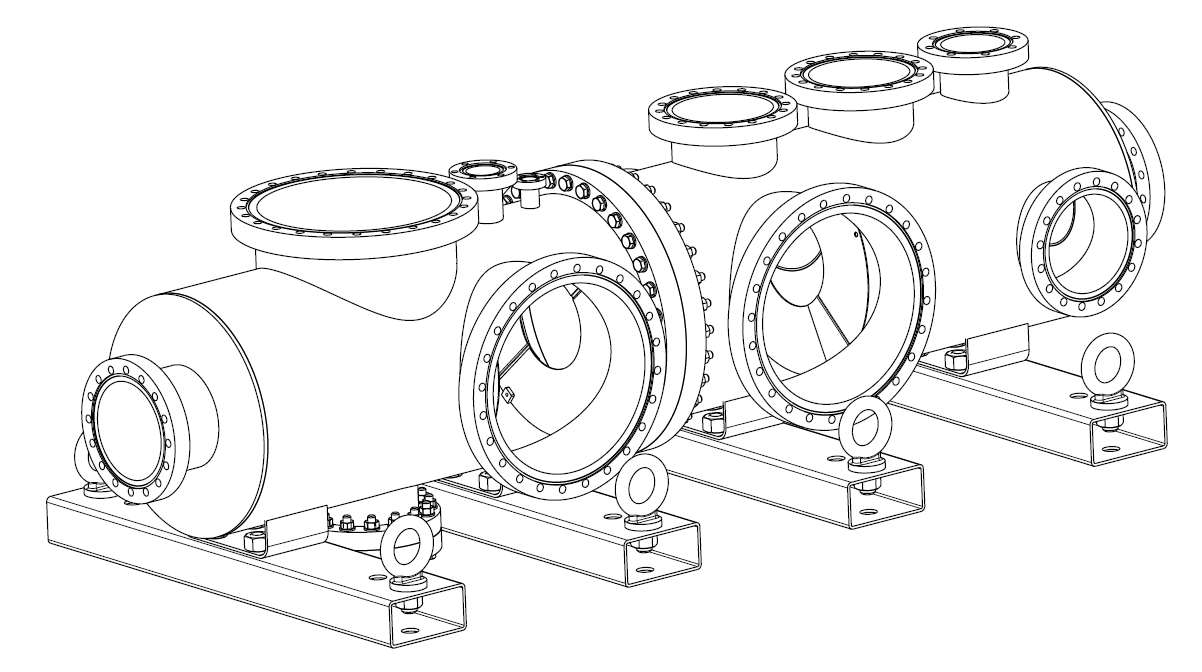
\includegraphics[width=\textwidth]{04_IPHI_Test/figures/fig000_Testbench.png}
	\end{center}
	\caption[IPM test bench]{IPM test bench. Left part is the LWU-like vessel
	while right part add more viewports for testing purposes.}
	\label{chap4:Testbench}
\end{figure}



  \subsection{Reference measurement [En cours de rédaction]}
  A reference measurement is alway a good practice when developing a detector. First, it may help to diagnostic possible issues on the prototypes. Then, it allows a complete comparison with the prototypes, and gives more confidence on the measurement. Therefore, two methods have been foreseen and implemented for this purpose.

  The first method uses scintillator screens, and thus is interceptive. The screens are mounted on a racket that can be inserted into the beam using a translator controlled remotely through a GEO BRICK controller. Three scintillator screens have been kindly provided by our colleagues at Saclay. Table \ref{chap4:tab_ecran} sums up the main characteristics of each screen, and Fig \ref{chap4:fig_ecran} shows the three screens on a support.

  The second system foreseen is a Fluorescence Profile Monitor (FPM). This system is developed by colleagues at ESS, indeed it will be the future NPM of the ESS MEBT. The FPM relies on a Image Intensifier (II) and a CMOS camera. An intensify image is a device that amplify visible photons. A photocathode on its input converts a incident photon into electrons. These electrons are then amplified by a single or double stages MCP and converted back into photons using a phosphor screen. Finally, a camera records the amplified image on the back of the phosphor screen. An II may detect a single photon as long as the incident photon is converted by the photocathode. However the information of the wavelength cannot be recover. The FPM is a totally non invasive method.


  \begin{wrapfigure}{r}{0.3\textwidth}
  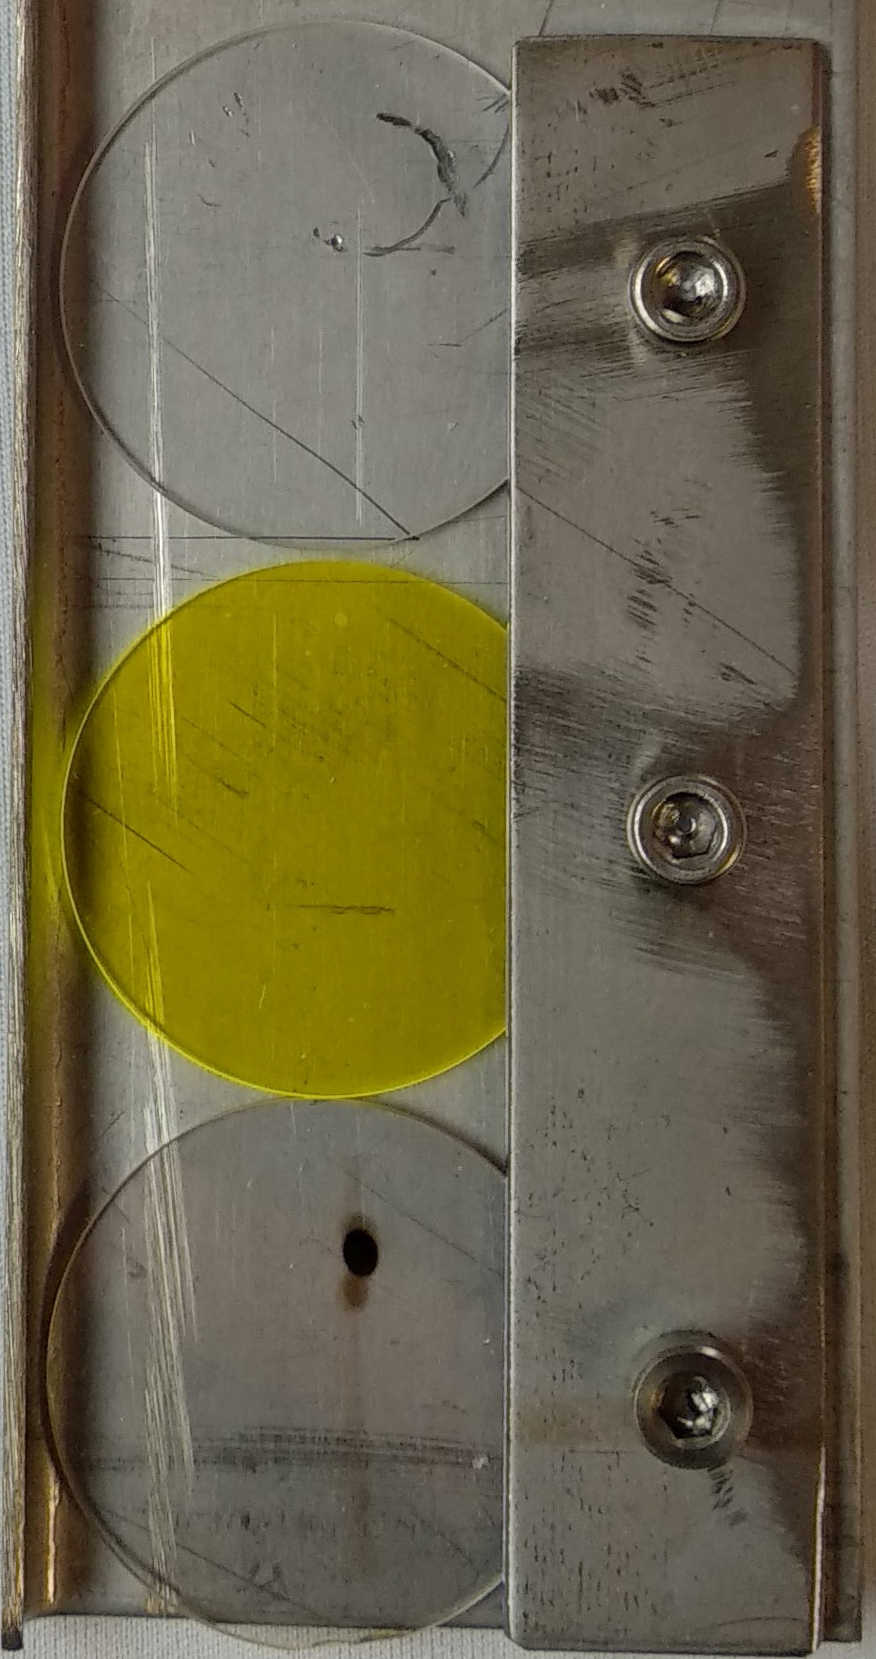
\includegraphics[width=0.3\textwidth]{04_IPHI_Test/figures/fig000_ecran.jpg}
  \caption[Picture of scintillator screen]{Picture of scintillator screen: Prelude420 (top), YAG:Ce (middle) and BGO (bottom).}
	\label{chap4:ecran}
\end{wrapfigure}

  \begin{table}[ht]
	\centering
	\caption[]{Properties common semiconductors used as radiation detector.}
	\label{chap3:semiconductor}
	\begin{tabular}{llll}
    \toprule
    Property & $\mathrm{Prelude}420$ $(Lu^{1.8}Y.^{2}SiO^{5}:Ce)$ & $\mathrm{YAG:Ce}$ & $\mathrm{CdTeZn}$ \\
    \midrule
    Density &  &  &  \\
    Light yield &  &  &  \\
    Typical wavelength &  & & \\
		\bottomrule
	\end{tabular}
\end{table}

  \section{IPHI test campaigns [En cours de rédaction]}
  \begin{figure}[!ht]
	\begin{subfigure}{0.5\textwidth}
		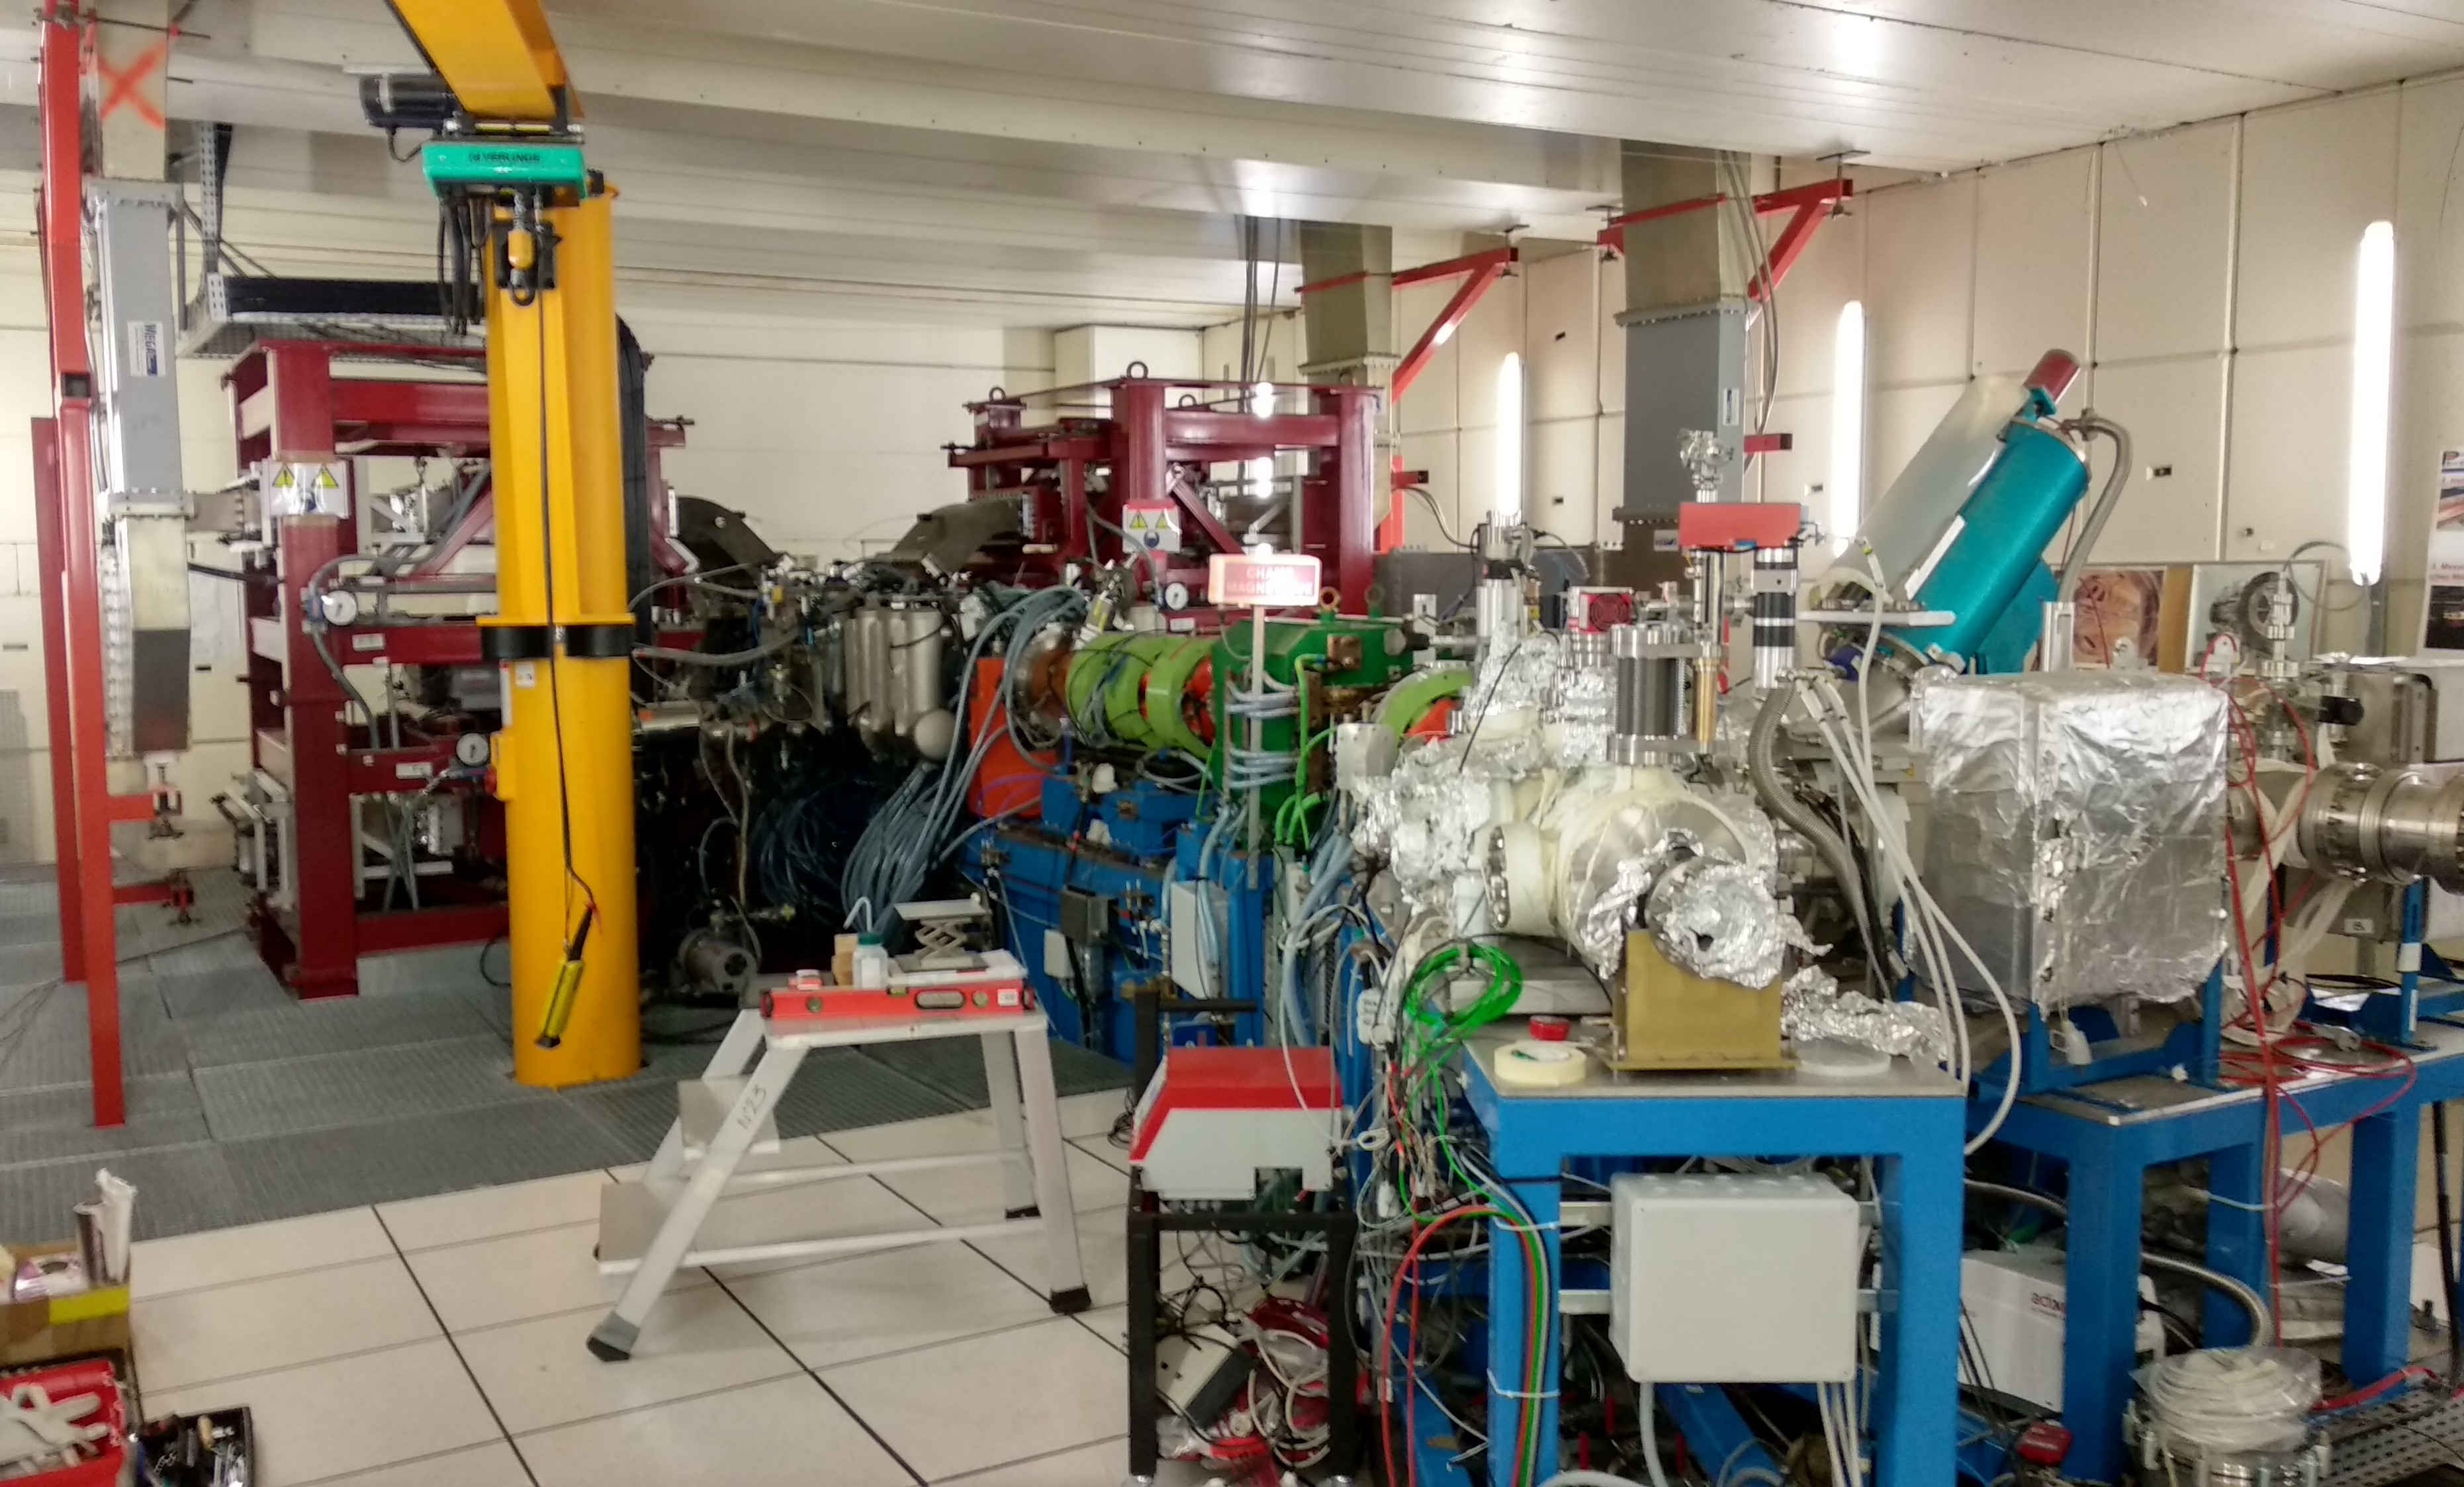
\includegraphics[width=\textwidth]{04_IPHI_Test/figures/fig000_IPHI_tb1.jpg}
		\caption{The casemate of IPHI. The test bench is visible in foreground}
		\label{}
	\end{subfigure}
	~
	\begin{subfigure}{0.5\textwidth}
		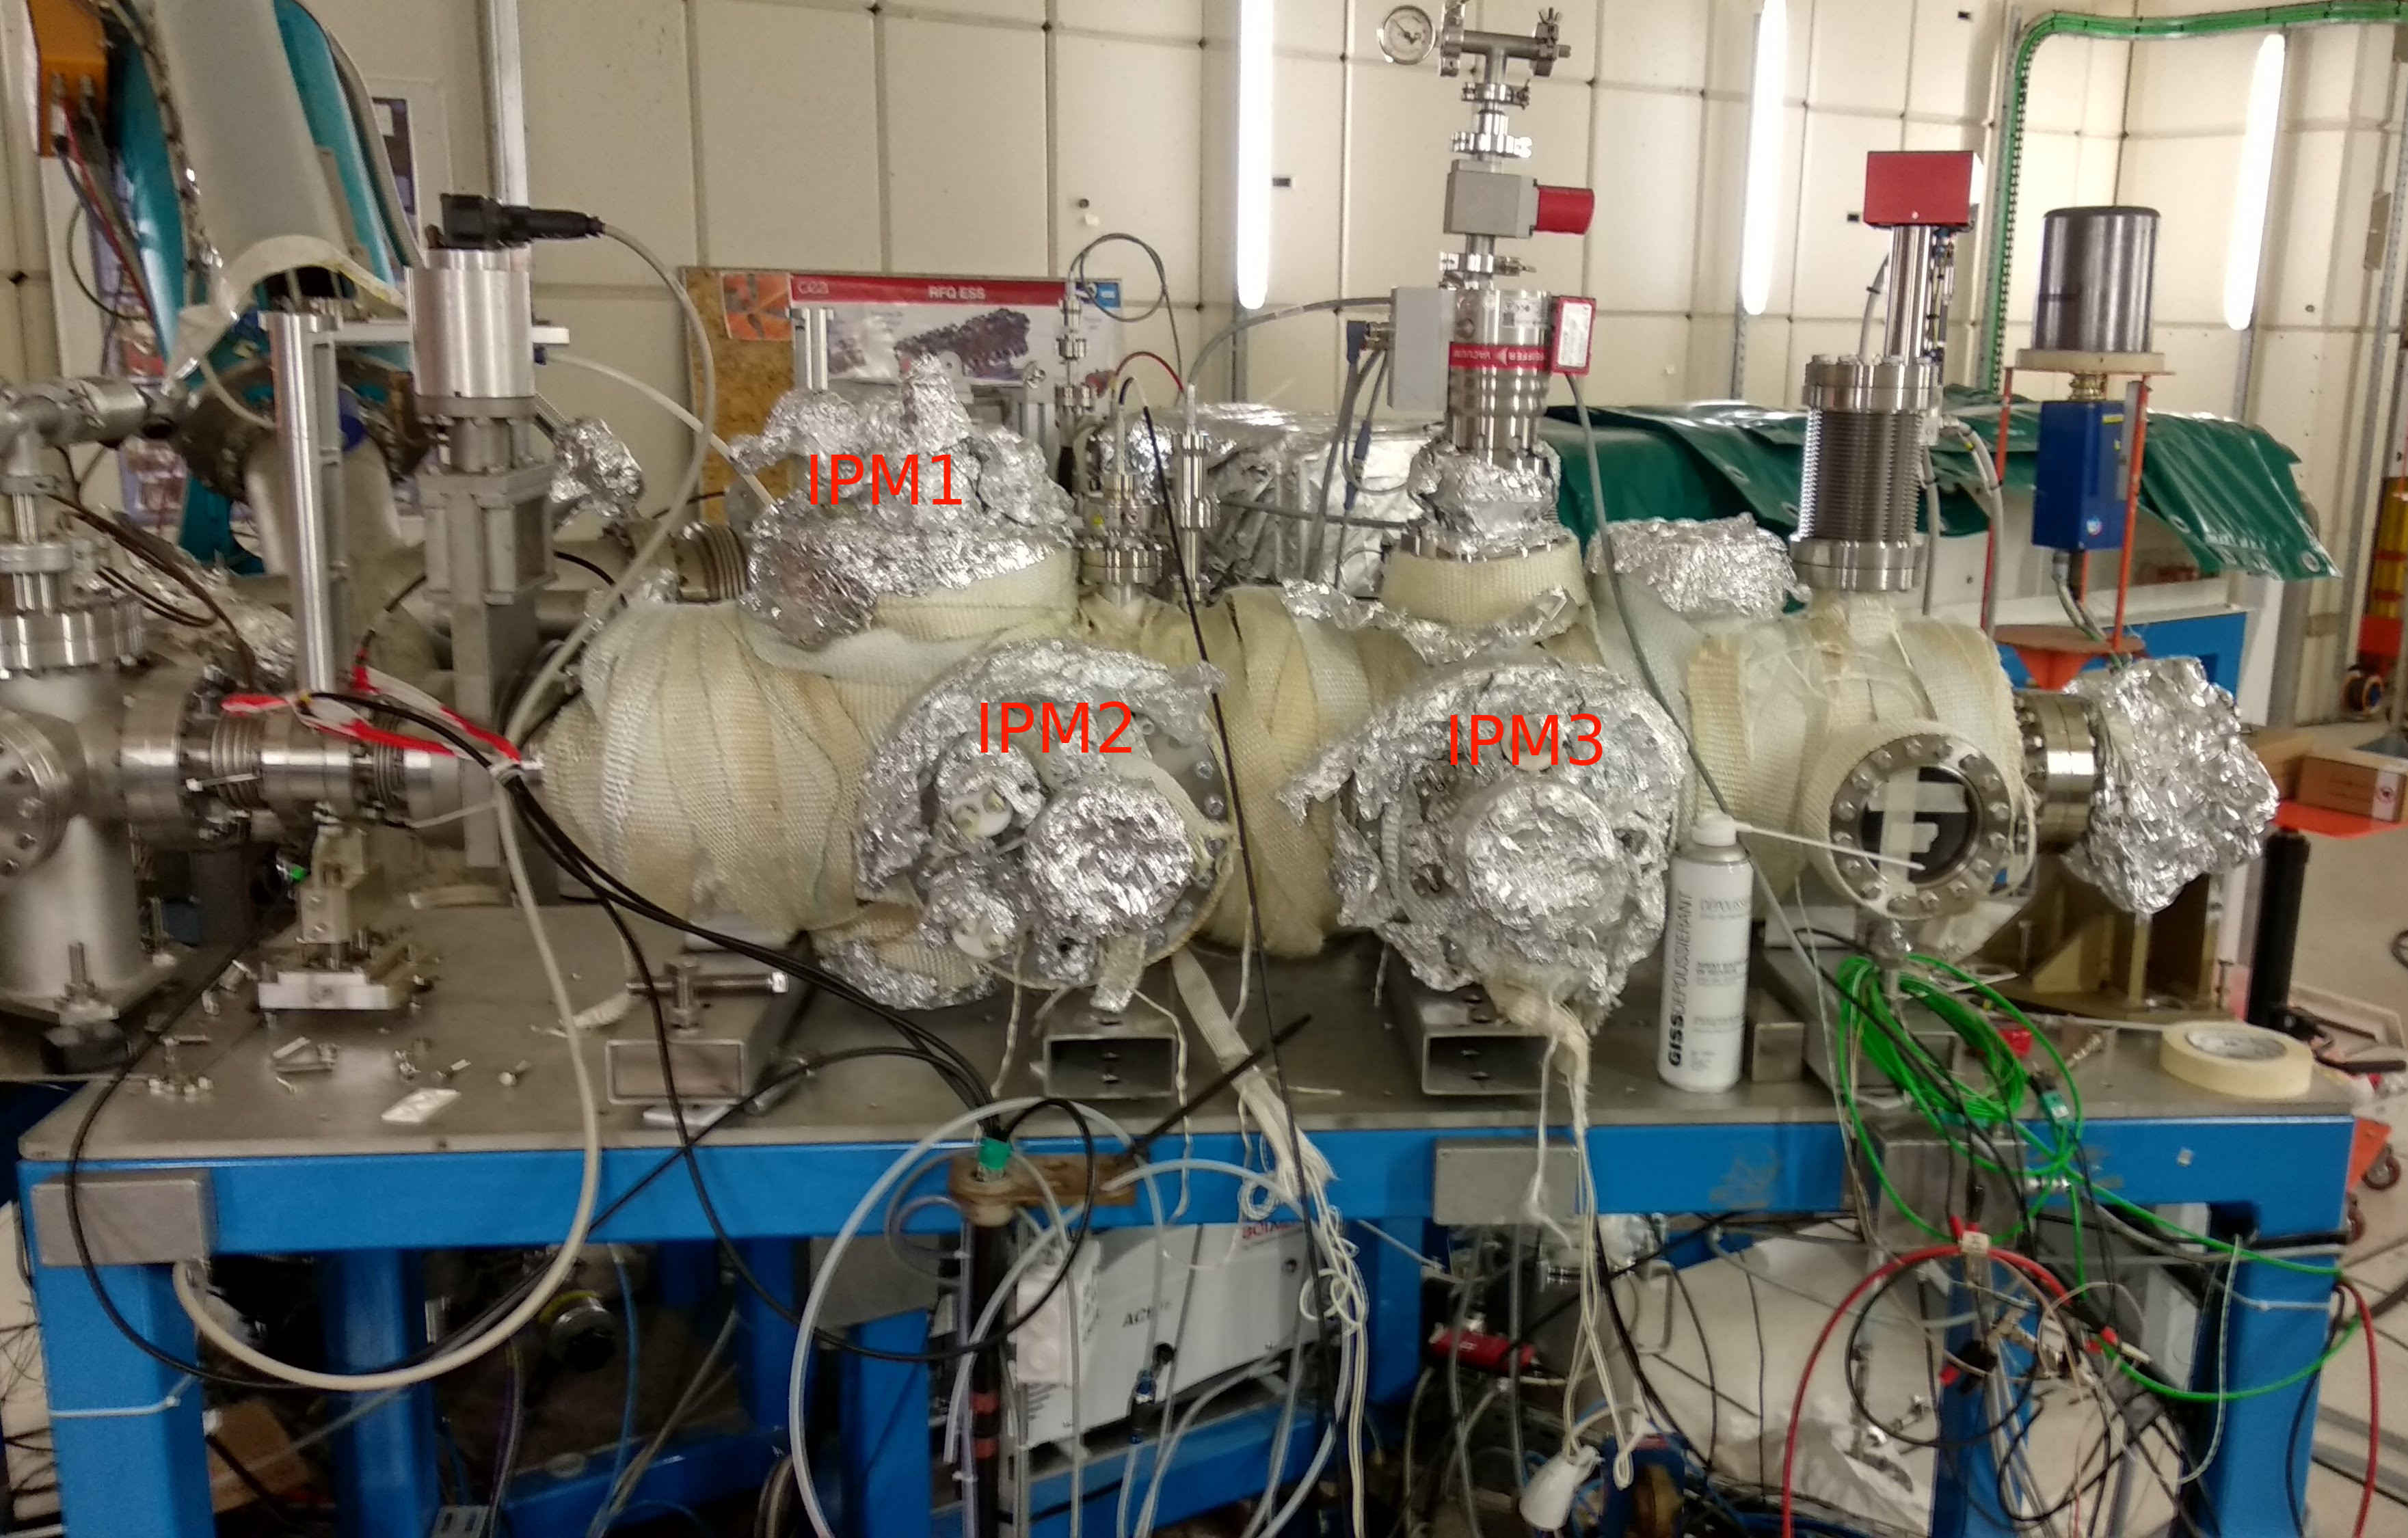
\includegraphics[width=\textwidth]{04_IPHI_Test/figures/fig000_IPHI_tb2.jpg}
		\caption{The test bench fully equipped.}
		\label{}
	\end{subfigure}
	\caption[The test bench installed at IPHI accelerator]{Th test bench installed at IPHI accelerator.}
	\label{chap4:IPHI_tb}
\end{figure}


  \subsection{IPHI accelerator [C]}
  IPHI is a high intensity linear proton accelerator located at CEA/Saclay.
  This project has been started in the late of 90's\cite{Beau2000} but protons were accelerated up to 3 MeV in April 2016\cite{Gobin2016}.

  Proton plasma is created by an electron cyclotron resonance source (ECR), and transported toward a radio frequency quadruple (RFQ) by a low energy beam transport line (LEBT).
  An iris assures a fine tuning of the current, and two solenoids focus and filter the plasma before the injection in the RFQ.
  Then, the protons are accelerated up to 3 MeV and bunched with a frequency of 352 MHz by the RFQ.
  A medium energy beam transport line (MEBT), downstream from the RFQ, contains focusing elements, steerers, dipole magnet and beam diagnostics.
  The dipole magnet can distribute the protons over two beam lines.

  The main line has a dedicated beam stop of 300 kW, allowing the commissioning of the accelerator at high intensity and duty cycle.
  The secondary line is more modular but restricted to lower intensity and duty cycle (few hundred Watts).
  This line is open for external user experiments.
  We were, with the nBLM team, one of the first experiments on the deviated line\cite{Senee:IPAC2018-TUPAF016}.

  Figure \ref{chap4:IPHI_view} shows schematic view of IPHI accelerator, and Table \ref{chap4:IPHI_carac} sums up difference between IPHI and ESS.

  \begin{figure}[!ht]
  \begin{center}
    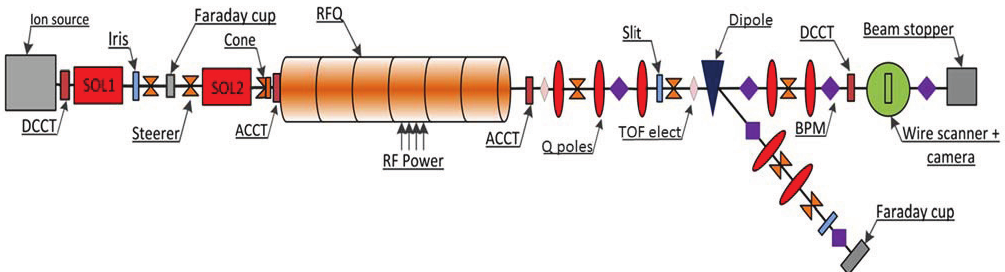
\includegraphics[width=\textwidth]{04_IPHI_Test/figures/fig000_IPHI_view.png}
  \end{center}
  \caption[Schematic view of IPHI accelerator]{Schematic view of the IPHI accelerator. The layout is almost up to date except that the slits have been removed. Our test bench was installed just after the last BPM on the deviated line.
    There is no other beam profiler measurement on this line.}
  \label{chap4:IPHI_view}
\end{figure}

  \begin{table}[!h]
  \centering
  \caption[Comparison between IPHI and ESS accelerators]{Comparison between IPHI and ESS accelerators.}
  \label{chap4:IPHI_carac}
  \begin{tabular}{lll}
    \toprule
                         & IPHI accelerator                                  & ESS accelerator                \\
    \midrule
    Energy               & $3\,\mathrm{MeV}$                                 & $2\,\mathrm{GeV}$              \\ \hline
    Max current          & $100\,\mathrm{mA}$                                & $62.5\,\mathrm{mA}$            \\ \hline
    Max pulse duration   & up to DC                                          & $2.86\,\mathrm{ms}$            \\ \hline
    Max pulse repetition & -                                                 & $14\,\mathrm{Hz}$              \\ \hline
    Vacuum range         & $5\cdot10^{-7}$ to $1\cdot10^{-8}\,\mathrm{mbar}$ & $1\cdot10^{-9}\,\mathrm{mbar}$ \\
    \bottomrule
  \end{tabular}
\end{table}

  \subsection{Setup [En cours de rédaction]}

  \section{Results [En cours de rédaction]}
  \subsection{Processing camera}
  \subsection{Processing strip}
  \cite{Brun1997,Antcheva2009}
  \subsection{Processing scintillator screen}
  \subsection{Review on the reference measurement}



  \subsection{Beam current}
  \subsection{Beam position}
  \subsection{Beam size and space charge}
  \subsection{Detection limits}
  \subsection{Comparison size}

  \section{COMSOL simulation}
  Simulations have been performed with COMSOL to cover both cases of asymmetric and symmetric configuration. The simulations expose a good uniformity with a  better result for symmetric configuration. However, it may be difficult to since the beam cannot be moved in a non uniform areas of the detector.
  
  A possible workaround consists in intentionally reduce the uniformity of the extraction, and the beam size and position will be more affected by non-uniformities. The optical IPM has been used in asymmetric configuration with a resistor chain designed for symmetric usage. Since resistor chains are different between asymmetric and symmetric configurations the extraction field will be also different. The electric field in this peculiar configuration can be simulated with COMSOL as shown previously.

  The three main effects have been observed from the simulations. Firstly, the beam image is smaller than the real beam size. This focusing effect is constant over the overall plane detection. Secondly, the extraction field tends to pull the beam image in the center of the detector. This effect is linear and null at the IPM center. Thus, the measured displacement is less important on the readout than the reality. Lastly, the beam image intensity is smaller in asymmetric because some particles are lost in the longitudinal direction. However, this effect can not be measured because the gain of MCP is not perfectly know on symmetric configure and cannot be recovered correctly.
  
  We measured the beam size and displacement for several steerer values in the symmetric and asymmetric configuration. The 
  The extractions field were set to same value for both configurations and all other parameters were frozen. If we suppose that the symmetric mode gives the real beam position and size, hence it is possible to quantify the difference between the simulations and experimental values.

  % TODO: Finir

  Note that the steerer was not able to cover the full range in position and we preferred to not use the dipole magnet to continue the scanning since it may affect the beam size.
  
  The method is clearly not perfect but it allows to reduce the IPHI uncertainty since it can be done without stopping down the accelerator.

  \subsection{Phosphorus screens}
  \subsubsection{Gain}
  % TODO: A améliorer
  A phosphorus screen converts a charged particle into visible photons.
  The signal amplitude depends on the energy deposition of the particle in the phosphorus layer. In our case, the phosphorus screen is placed just after the MCP output. So the signal is proportional to the accelerating voltage between the MCP output and the phosphorus screen. Two screens have been tested during the beam tests: the P43 and the P46. Each screen has its intrinsic characteristics like the yield, the emission wavelength and the decay time. Fig. \ref{fig:phos_integral} expose the linear response with the voltage for both the screens. The beam size seems to be not affected by the screen gain, as shown in Fig. \ref{fig:phos_pos}. According to Hamamatsu, the lifetime of a phosphorus screen is negligible with respect to the MCP lifetime.

  \begin{figure}[!ht]
	\begin{subfigure}[t]{0.5\textwidth}
		\includesvg[width=\textwidth]{04_IPHI_Test/figures/fig000_P43_size.svg}
		\caption{P43 screen.}
		\label{}
	\end{subfigure}
	~
	\begin{subfigure}[t]{0.5\textwidth}
		\includesvg[width=\textwidth]{04_IPHI_Test/figures/fig000_P46_size.svg}
		\caption{P46 screen.}
		\label{}
	\end{subfigure}
	\caption[Beam size versus phosphorus screen voltage.]{Beam size versus phosphorus screen voltage. No significant change of the beam size has been observed.}
	\label{chap4:P_size}
\end{figure}

  \begin{figure}[!ht]
	\begin{subfigure}{0.5\textwidth}
		\includesvg[width=\textwidth]{04_IPHI_Test/figures/fig000_P43_gain.svg}
		\caption{}
		\label{}
	\end{subfigure}
	~
	\begin{subfigure}{0.5\textwidth}
		\includesvg[width=\textwidth]{04_IPHI_Test/figures/fig000_P46_gain.svg}
		\caption{}
		\label{}
	\end{subfigure}
	\caption[]{}
	\label{chap4:P_gain}
\end{figure}

  \subsubsection{Timing}
  % TODO: A améliorer
  The measurement of decay time has been performed by moving the camera trigger at small exposure times. The measurement is a bit more difficult for the fast screen. Indeed, the exposure time is now comparable to the decay time, also the delay and the jitter on the exposure time may afflict the measurement. As expected, the P43 is slow, thus if this screen is used for ESS then the total integration time on camera should be set to $10\,\mathrm{ms}$ and not strictly to $2.86\,\mathrm{ms}$ ms. This is not the case with the P46 screen.
  \begin{figure}[!ht]
	\begin{subfigure}{0.5\textwidth}
		\includesvg[width=\textwidth]{04_IPHI_Test/figures/fig000_P43_timing.svg}
		\caption{}
		\label{}
	\end{subfigure}
	~
	\begin{subfigure}{0.5\textwidth}
		\includesvg[width=\textwidth]{04_IPHI_Test/figures/fig000_P46_timing.svg}
		\caption{}
		\label{}
	\end{subfigure}
	\caption[]{}
	\label{chap4:P_timing}
\end{figure}

  \subsection{Extrapolation to ESS condition}
  Unlike the strips IPM, it is almost impossible to quantify the number of ionization particles without a full calibration of the MCPs. Hence, the extrapolation to ESS conditions is only done from Bethe Bloch formula, with respect to the beam parameters and vacuum conditions measured at IPHI. We supposed that the signal scales linearly with pressure. The beam current and the pulse duration were set to their lowest value possible at IPHI, respectively $0.7\,\mathrm{mA}$ and 50 $50\, \mathrm{\mu s}$. The vacuum level was about $4 \cdot 10^{-8}\,\mathrm{mbar}$ and its composition was mainly water (conservative assumption), see Appendix \ref{app:RGA}. Table \ref{tab:ESS_extrapolation} sums up the factor of each parameter on the extrapolation. At first glance, it seems to be possible to measure single profile at nominal ESS conditions. However, this assumption is strongly dependent to the vacuum conditions. Neither the RGA nor the gauges were calibrated so the uncertainty may be relevant.
  \begin{table}[ht]
  \centering
  \caption[Extrapolation to ESS conditions from a real case during the second campaign]
  {Extrapolation to ESS conditions from a real case during the second campaign.
    The IPHI current was below $0.7\,\mathrm{mA}$ with a pulse duration of $50\, \mathrm{\mu s}$. Pressure level was $4 \cdot 10^{-8}\,\mathrm{mbar}$ with mainly water vapors (conservative hypothesis).
    The scaling factor for each parameter is calculated from the nominal ESS beam conditions given in Table \ref{chap2:ess_charac}.}
  \label{chap4:extrapolationMCP}
  \begin{tabularx}{\linewidth}{XXXXXXX}
    \toprule    ESS energy (MeV) & Bethe Bloch & Pressure     & Gas composition & Intensity & Pulse length & Total         \\
    \midrule
    \(97.2\)                     & $\times 15.5$ & $\times 40 $ & $\times 2.2$    & $\div89$  & $\div57$     & $\times 0.27$ \\
    \(231.4\)                    & $\times 16.4$ & $\times 40$  & $\times 2.2$    & $\div89$  & $\div57$     & $\times 0.28$ \\
    \(278.9\)                    & $\times 29.9$ & $\times 40$  & $\times 2.2$    & $\div89$  & $\div57$     & $\times 0.52$ \\
    \(315.8\)                    & $\times 33.4$ & $\times 40$  & $\times 2.2$    & $\div89$  & $\div57$     & $\times 0.58$ \\
    \(628.3\)                    & $\times 35.8$ & $\times 40$  & $\times 2.2$    & $\div89$  & $\div57$     & $\times 0.62$ \\
    \bottomrule
  \end{tabularx}
\end{table}

  \subsection{Electron measurement with MCP}
  Unfortunately, we were not able to measure any profile in electron mode during the first and second campaign.
  Typical pictures in the electron configuration are shown in Figure \ref{fig:electron}. One can see that the . A higher signal is observed on the sides of the MCPs.
  The MCPs are in general a little less sensitive to electrons compare to ions at energies between five and ten keV \cite{Wiza1979}.
  However, during tests the signal on the camera was always far higher for electrons without any modifications of the gain or the beam conditions.
  Hence, we suppose that the electron background is huge at IPHI.
  During tests, permanent magnets have been installed close to the aperture and beam dump. No clearly improvements have been observed. We still don't know exactly why there is so many electrons.
  \begin{figure}[!ht]
	\begin{subfigure}[t]{0.5\textwidth}
		\includesvg[width=\textwidth]{04_IPHI_Test/figures/fig000_electron_Hamamatsu.svg}
		\caption{Profile measurement attempt with electrons, Hamamatsu MCP.}
		\label{}
	\end{subfigure}
	~
	\begin{subfigure}[t]{0.5\textwidth}
		\includesvg[width=\textwidth]{04_IPHI_Test/figures/fig000_electron_Photonis.svg}
		\caption{Profile measurement attempt with electrons, Photonis MCP.}
		\label{}
	\end{subfigure}
	\caption[Example of images in electron mode]{Example of images in electron mode for both MCPs.
  Some patterns seem to be the same in the edges and middle of the images.
  The line in the middle is not correlated with the beam.}
	\label{chap4:electron_MCP}
\end{figure}


  \section{Summary [En cours de rédaction]}
  \label{ch4:Summary}

  \cleardoublepage
  \section{Bibliography}
  \label{ch4:bib}
  \printbibliography[heading=subbibliography]

\end{refsection}